\documentclass[11pt]{article}

%────────────────────────────────────────────────
%— Your existing style
\usepackage{pepadun}
\usepackage{float}
\usepackage{xcolor}
\usepackage{color}
\usepackage{soul}
\usepackage{hyperref}


\usepackage[T1]{fontenc}
\usepackage{listings}
\usepackage{xcolor} 
%\usepackage{minted}

\usepackage{graphicx}%
\usepackage{multirow}%
\usepackage{amsmath,amssymb,amsfonts}%
\usepackage{amsthm}%
\usepackage{mathrsfs}%
\usepackage[title]{appendix}%
\usepackage{xcolor}%
\usepackage{textcomp}%
\usepackage{manyfoot}%
\usepackage{booktabs}%
\usepackage{float}
\usepackage{hyperref}
\usepackage{calrsfs}

\usepackage{listings}%
\usepackage{caption}
\usepackage{subcaption}

%\usepackage{amsmath,amsfonts,amsbsy,amssymb,amsthm,mathtools,tabulary,graphicx,caption,fancyhdr, mathrsfs, pgf, pgfplots, epsfig, epstopdf, lscape,booktabs,enumitem,lipsum,tkz-graph,scalerel,stackengine,setspace,adjustbox,float,amsthm}
%\usepackage[labelformat=simple]{subfig}
%\renewcommand\thesubfigure{\normalfont(\textbf{\alph{subfigure}})}

\definecolor{solBlue}   {HTML}{268BD2}	% keyword / function
%\colorlet{darkgreen}{green!50!black!75}	% strings
\definecolor{darkgreen}{HTML}{2E7D32}

% Define a simple style
\lstdefinestyle{mystyle}{
  basicstyle=\ttfamily\small,
  keywordstyle=\color{solBlue},
  commentstyle=\color{gray},
  stringstyle=\color{darkgreen},
  frame=single,
  numbers=left,
  numberstyle=\tiny,
  breaklines=true
}
\lstset{style=mystyle}






%────────────────────────────────────────────────
%— BIBLIOGRAPHY SETUP (biblatex + Biber)
\usepackage[backend=biber,style=ieee]{biblatex}
\addbibresource{pepadun.bib}
% Uncomment to include _all_ entries from pepadun.bib, even if not cited:
\nocite{*}

%────────────────────────────────────────────────
\title{Designing an Interactive, Reproducible Statistics E-Book: A Student–Faculty Collaboration Using Bookdown and R}
\author{%
    \begin{tabular}{c}
        \textsuperscript{1}Nurlana Alili and\\
        \textsuperscript{2}Bryan Xu \\[6pt]
        \textsuperscript{1,2} Department of Mathematical and Computational Sciences, University of Toronto Mississauga, \\ 
        3359 Mississauga Road, Mississauga ON, L5M 3Z3\\[6pt]
        e-mail: \textsuperscript{1} \href{mailto:nurlana.alili@mail.utoronto.ca}{\uline{nurlana.alili@mail.utoronto.ca}}\\
        \textsuperscript{2} \href{mailto:bryansuxi.su@mail.utoronto.ca}{\uline{bryansuxi.su@mail.utoronto.ca}}
    \end{tabular}%
}
\date{}

\begin{document}

\maketitle

\begin{abstract}
%Most undergraduate students are introduced to statistics through lectures and textbooks that emphasize theoretical knowledge but offer limited opportunities for active learning or applied practice. In this project, we collaborated with faculty to develop an interactive, open-access e-book designed to integrate statistical theory with hands-on analytical practice. The resource combines step-by-step explanations with embedded code examples, data-driven graphics, and user-controlled simulations to encourage exploratory and applied learning.
%
%Initially developed in LaTeX, the project was later transitioned to the Bookdown framework to improve accessibility, interactivity, and reproducibility. Content was reorganized to improve instructional flow, and the visual and interactive elements were developed using R-based tools such as ggplot2 and Shiny. GitHub and GitHub Pages facilitated version control, collaborative authorship, and online publishing.
%
%The project illustrates the contributions of students to curricular innovation in the development of educational resources. Participating in the design and technical implementation deepened our own learning while producing a tool that can benefit future learners. It also highlights the potential of open-source technologies and student–faculty collaboration to support the development of inclusive, adaptive, and accessible resources for statistical education.

In most university courses, students learn from textbooks they did not help develop. 
We present an innovative approach where undergraduate students collaborated with faculty to create an open-access, interactive web-based e-book for an introductory applied statistics course.
%This process allows undergraduate students to be co-authors rather than passive readers, fostering an appreciation for reproducible research, provides opportunities for collaboration, learning about project management and work flows, and gaining opportunities to independently learn and apply new skills and technologies.
This process transforms undergraduates into co-authors rather than passive readers, fosters an appreciation for reproducible research, encourages academic collaboration, and offers hands-on opportunities to acquire and apply new skills and technologies.
Faculty also benefit from fresh ideas and new perspectives.
This type of collaboration is important to explore since evidence on student--faculty partnerships on developing course materials is sparse in the literature, particularly in a Canadian context and in the area of statistics.
%To address this, we collaborated with faculty to develop and contribute to developing a live, interactive e-book for an applied statistics course at the University of Toronto Mississauga.
In this paper, we illustrate the contributions of undergraduate students to curricular innovation in the development of the e-book by describing the development process, methodology and software tools used, and reflect on our experience in the process of being collaborators alongside faculty.
Our participation deepened our own learning while producing resources to benefit future learners, we highlight the potential of open-source technologies and student–faculty collaboration to support the development of inclusive, adaptive, and accessible resources for statistical education.

\keywords{Bookdown, Shiny, Plotly, GitHub pages, Statistics education}

\end{abstract}

\section{INTRODUCTION}

Undergraduate courses designed through a partnership between faculty and students can deepen engagement and develop a meaningful learning experience \cite{Healey2016,Bovill2019}. 
Students are provided with the opportunity to be co-creators, rather than simply passive recipients of information, thereby encouraging them to take ownership of their educational journey, and faculty gain fresh insights into how students learn \cite{Healey2016}.
These partnerships between deepen engagement and promote more authentic learning experiences for both students and faculty involved \cite{Healey2016,Bengtson2013}.
Systematic reviews highlight that such collaborations enhance motivation, empower students, and enrich teaching practice, yet they have not been studied or documented uniformly across disciplines \cite{MercerMapstone2017,Bovill2019} and reports of whole-course co-creation are particularly limited within statistics education \cite{Kim2022}. 
Systematic reviews by Mercer et.al \cite{MercerMapstone2017} and Omland et. al discuss several studies where students and faculty have partnered in course designed internationally, however there is a lack of such collaboration documents in relation to mathematics and statistics education \cite{Duah2011}.
To the best of our knowledge, we could not find any collaborations specifically in a Canadian context.

Furthermore, many undergraduate statistics courses introduce foundational concepts through traditional lectures and texts. 
Even digital versions of textbooks are still usually static with limited advantages beyond quickly searching for content and conveniently applying bookmarks.
While these approaches build necessary theoretical understanding, they are often unable to provide opportunities for students to interact meaningfully with statistical methods or explore real-world applications. 
Topics such as hypothesis testing, confidence intervals, and regression frequently may remain abstract due to limited context and passive delivery formats  
\colorbox{yellow!34}{\textcolor{red}{\textbf{[PLEASE FIND CITATION TO JUSTIFY THIS]}}}.


Our project emerged in response to those to the lack of study in student-faculty collaboration in co-developing course material and to simultaneously address the limitations of traditional texts in statistics. 
We partnered with faculty through the \textit{STA378: Independent Research Project Course}, at the University of Toronto Mississauga (UTM) to assist the current course coordinator, Professor Nishan Mudalige, for \textit{STA258: Statistics with Applied Probability}, develop an interactive e-book for the course as part of an on-going course redevelopment project.
STA258 is an introductory applied statistics course at UTM where most students are learn about applied inference techniques (i.e. testing of hypotheses, interval estimation) and regression for the first time in their university learning experience.
This is an important course since it provides students with the foundational skills for data analysis and equips them with the ability to interpret statistical results in advanced courses across all disciplines, including other statistics courses, the life sciences, social sciences, economics and finance and computer science courses requiring a knowledge of inference.
This course also provides students with the ability to read and interpret statistical results from academic journals which is essential for critically evaluating research, making evidence-based decisions, and succeeding in advanced study and professional practice in both academic and non-academic settings.

Dr. Mudalige is involved in a long term project to redesign the content in STA258. 
There are several reasons justifying the development of STA258.
One such reason is that it currently overlaps considerably with \textit{STA260: Probability and Statistics II}, with both courses sharing common introductory content.
Students simultaneously enrolled in both courses experience substantial duplication in the content delivered to them during the opening weeks of both courses.
Another reason to redevelop STA258 is the necessity to incorporate more data analysis components to modernize the course and make it more relevant for students by equipping them with foundational skills for independent statistical analysis.
There some distinct features of STA258 which makes it a good candidate for collaborative re-design between students and faculty.
Within the University of Toronto system, STA258 is only offered at the Mississauga campus and there is no equivalent course or combination of courses available at the St. George campus or the Scarborough campus.
Therefore, it has the potential to be a self-contained course which can equip students with the skills required providing an efficient pathway for students to learn important skills related to statistical reasoning, which is equivalent to multiple courses from other campuses, 
Redesigning STA258 eliminates the necessity for the Department of Mathematical and Computational Sciences at UTM to go through lengthy development and approval process required for an entirely new course to address the curricular gap.

During the initial phase of the STA258 course development timeline, we as undergraduate students worked alongside Dr. Mudalige and Dr. Ataei to produce an open-access, interactive e-book which integrates narrative exposition, reproducible simulations and examples involving code, embeds visualizations and interactive components to explain concepts, and provides an open-source resource for educators in the broader statistical community.
This paper outlines the framework that guided our partnership, describes the authoring workflow (version control, peer review, and continuous deployment), and reflects on early outcomes. By sharing these first-phase results, we aim to provide a practical model for implementing student-faculty co-creation in applied statistics and related quantitative courses.

%In summer 2025, a collaborative initiative between undergraduate students and faculty sought to restructure the delivery of statistical content through an interactive, web-based e-book. The objective was to develop a resource that not only explained statistical theory, but also incorporated dynamic learning tools—including live code, responsive graphics, and simulation-based applications—to enhance student engagement and agency.
%
%Drawing on our own experiences as learners, we envisioned a platform that would support exploratory learning, offer clearer explanations, and foster reproducible practices. From the outset, the project was guided by principles of open access, collaboration, and technical transparency, with the intention that the resulting e-book would serve both current students and the broader educational community.
%
%The live version of the interactive e-book is available at: \url{https://nishanmudalige.github.io/STA258}.


\section{DESIGN, DEVELOPMENT AND IMPLEMENTATION}

The core team consisted of two undergraduate students, Nurlana Alili and Xi Su, who contributed to both content development and technical implementation. Professors Nishan Mudalige and Masoud Ataei provided consistent guidance through regular meetings, detailed feedback, training with software, and contributed critical input into decisions regarding the e-book’s structure and tools.
Both Professors also assisted with trouble shooting and Professors Nishan contributed a substantial amount towards the coding component, particularly with initiating the framework and resolving some of the more challenging components.
We also received valuable external feedback from Dr. Steve Tully, Mathematics Professor at Okanagan College, and Avanti Coonghe, Communications and Design Consultant at the United Nations (World Health Organization), who provided suggestions related to content scope, pedagogical structure, and overall educational value.

The interactive e-book project was launched in Summer 2025 semester as a joint initiative between undergraduate students and faculty to create an engaging and innovative learning resource for students enrolled in statistics courses. 
The University of Toronto Mississauga provides high-performing undergraduate students enrolled in a statistics major or specialist with the opportunity to enrol in \textit{STA378: Statistics Research Project}, where students explore a topic in statistics under the supervision of a faculty member.
Students can not directly enrol into STA378 through ACORN, and a special administrative process is required, including approval from the associate chair.
Both authors of this paper had recently completed STA258 during the Winter 2025 semester and agreed with Dr. Mudalige that the course required adjustments, and we mutually expressed interest in working together on this course redevelopment project.

Our initial decision was to use LaTeX to create a Portable Document Format (PDF) e-book.
This was based on its well-established typesetting capabilities and familiarity within academic publishing.
This PDF document generate in LaTeX is also easily accessible on many devices.
In addition, open-source resources, such as OpenIntro Statistics, which offer an extensive material to utilize as a foundation to develop an e-book using LaTeX.
However there are limitations with this approach, including being limited to fixed sized pages to display content, limited navigation options, the difficulty with embedding interactive components, and maintaining an organized working environment due to the many auxiliary files produced.

Although we began the e-book in LaTeX, midway through our development we learned about Bookdown which is a package in R package developed for writing materials such as books and long-form content with R Markdown. 
Bookdown has the advantage of converting R Markdown into responsive HTML, EPUB, and print-ready PDF while automatically generating cross-references and a searchable table of contents, LaTeX can be typeset within R Markdown documents, the HTML output from Bookdown can embed live R code, interactive widgets, and interactive apps using libraries such as shiny and plotly, giving students a hands-on e-book experience that fixed-layout PDFs cannot match, and a book generated in Bookdown can be hosted on GitHub pages allowing anyone with an internet connection to easily access it.
Due to its many advantages over traditional LaTeX, we decided to transition to the Bookdown framework since it proved more compatible with the goals of interactive and accessible online learning. 

This shift from LaTex to Bookdown allowed us to integrate dynamic and interactive elements that enhance student engagement and understanding and
%More importantly, Bookdown offered key features such as inline code execution, interactive graphics, and dynamic cross-referencing of equations, figures, and tables—transforming static content into a fully interactive learning resource.
transformed static content into a fully interactive learning resource.
The conversion from LaTeX (.tex) to R Markdown (.Rmd) was performed using Pandoc, with the majority of the the formatting and structure intact. Pandoc also preserved most of the fidelity of the LaTeX code during the conversion. 
The syntax used for the conversion is given in Listings \ref{lst:tex_to_rmd_basic} and \ref{lst:tex_to_rmd_mathjax}.\\

\begin{lstlisting}[language=bash,
                   caption={Basic conversion of a LaTeX .tex file to an R Markdown .Rmd file using Pandoc},
                   label={lst:tex_to_rmd_basic},
                   captionpos=b] 
pandoc -s input.tex -f latex -t markdown -o output.Rmd
\end{lstlisting}

\hfill

\begin{lstlisting}[language=bash,
                   caption={Conversion of a LaTeX .tex file to an R Markdown .Rmd file rendered with MathJax using Pandoc},
                   label={lst:tex_to_rmd_mathjax},
                   captionpos=b] 
pandoc --filter pandoc-citeproc --mathjax -s input.tex -f latex -t markdown -o output.Rmd
\end{lstlisting}

Once we established our framework, we selected other open-source tools and programming languages that could support both visual design and reproducible workflows around Bookdown. A summary of the technologies used in developing the e-book are listed in Table \ref{tab:ebook_Technologies}.

\renewcommand\arraystretch{1.25}
\begin{table}[H]
\setlength{\belowcaptionskip}{-20pt}
\begin{center}
\begin{tabular}{| l | l |}
\hline
\textbf{Languages}		&	R, R Markdown, LaTeX, YAML, HTML, CSS, JavaScript\\
\hline
\textbf{Frameworks} 		&	Bookdown, R Markdown\\
\hline
\textbf{R packages}		&	knitr, ggplot2, plotly, Shiny, rgl\\
\hline
\textbf{Version Control} 	&	GitHub, GitHub Pages \\
\hline
\textbf{Deployment} 		&	GitHub Pages \\
\hline
\end{tabular}
\caption{Summary of software, libraries and frameworks used in developing the e-book.}
\label{tab:ebook_Technologies}
\end{center}
\end{table}
\renewcommand\arraystretch{1.00}

The tools utilized in Table \ref{tab:ebook_Technologies} were intentionally selected for their compatibility, transparency, and capacity to support reproducible computing. 
Some tools were used directly such as R Markdown and R, while others were secondary technologies which were used by the frameworks in rendering the e-book.
GitHub served both as a collaborative development platform and as a public-facing repository for version control, while GitHub Pages enabled open access to the live e-book and supported asynchronous contributions from others.
The YAML file was used for front matter, to store the book’s metadata, for build settings and for integration with GitHub pages.
CSS was used to customize environments in Bookdown, such as the definition environment and remark environment with personalized aesthetics and consistent colour scheme.

Although we encountered some technical challenges, especially during the transition from LaTeX to Bookdown, these obstacles deepened our understanding of collaborative digital authorship and reproducible research. The final product represents not only an innovative approach to content delivery, but also an exploration of what collaborative educational development can look like in practice.

%\begin{pepadunfigure}{GitHub repository structure showing organized files, collaborative development history, and team contributions for the e-book project. GitHub supported version control, content management, and public access through GitHub Pages.}
%    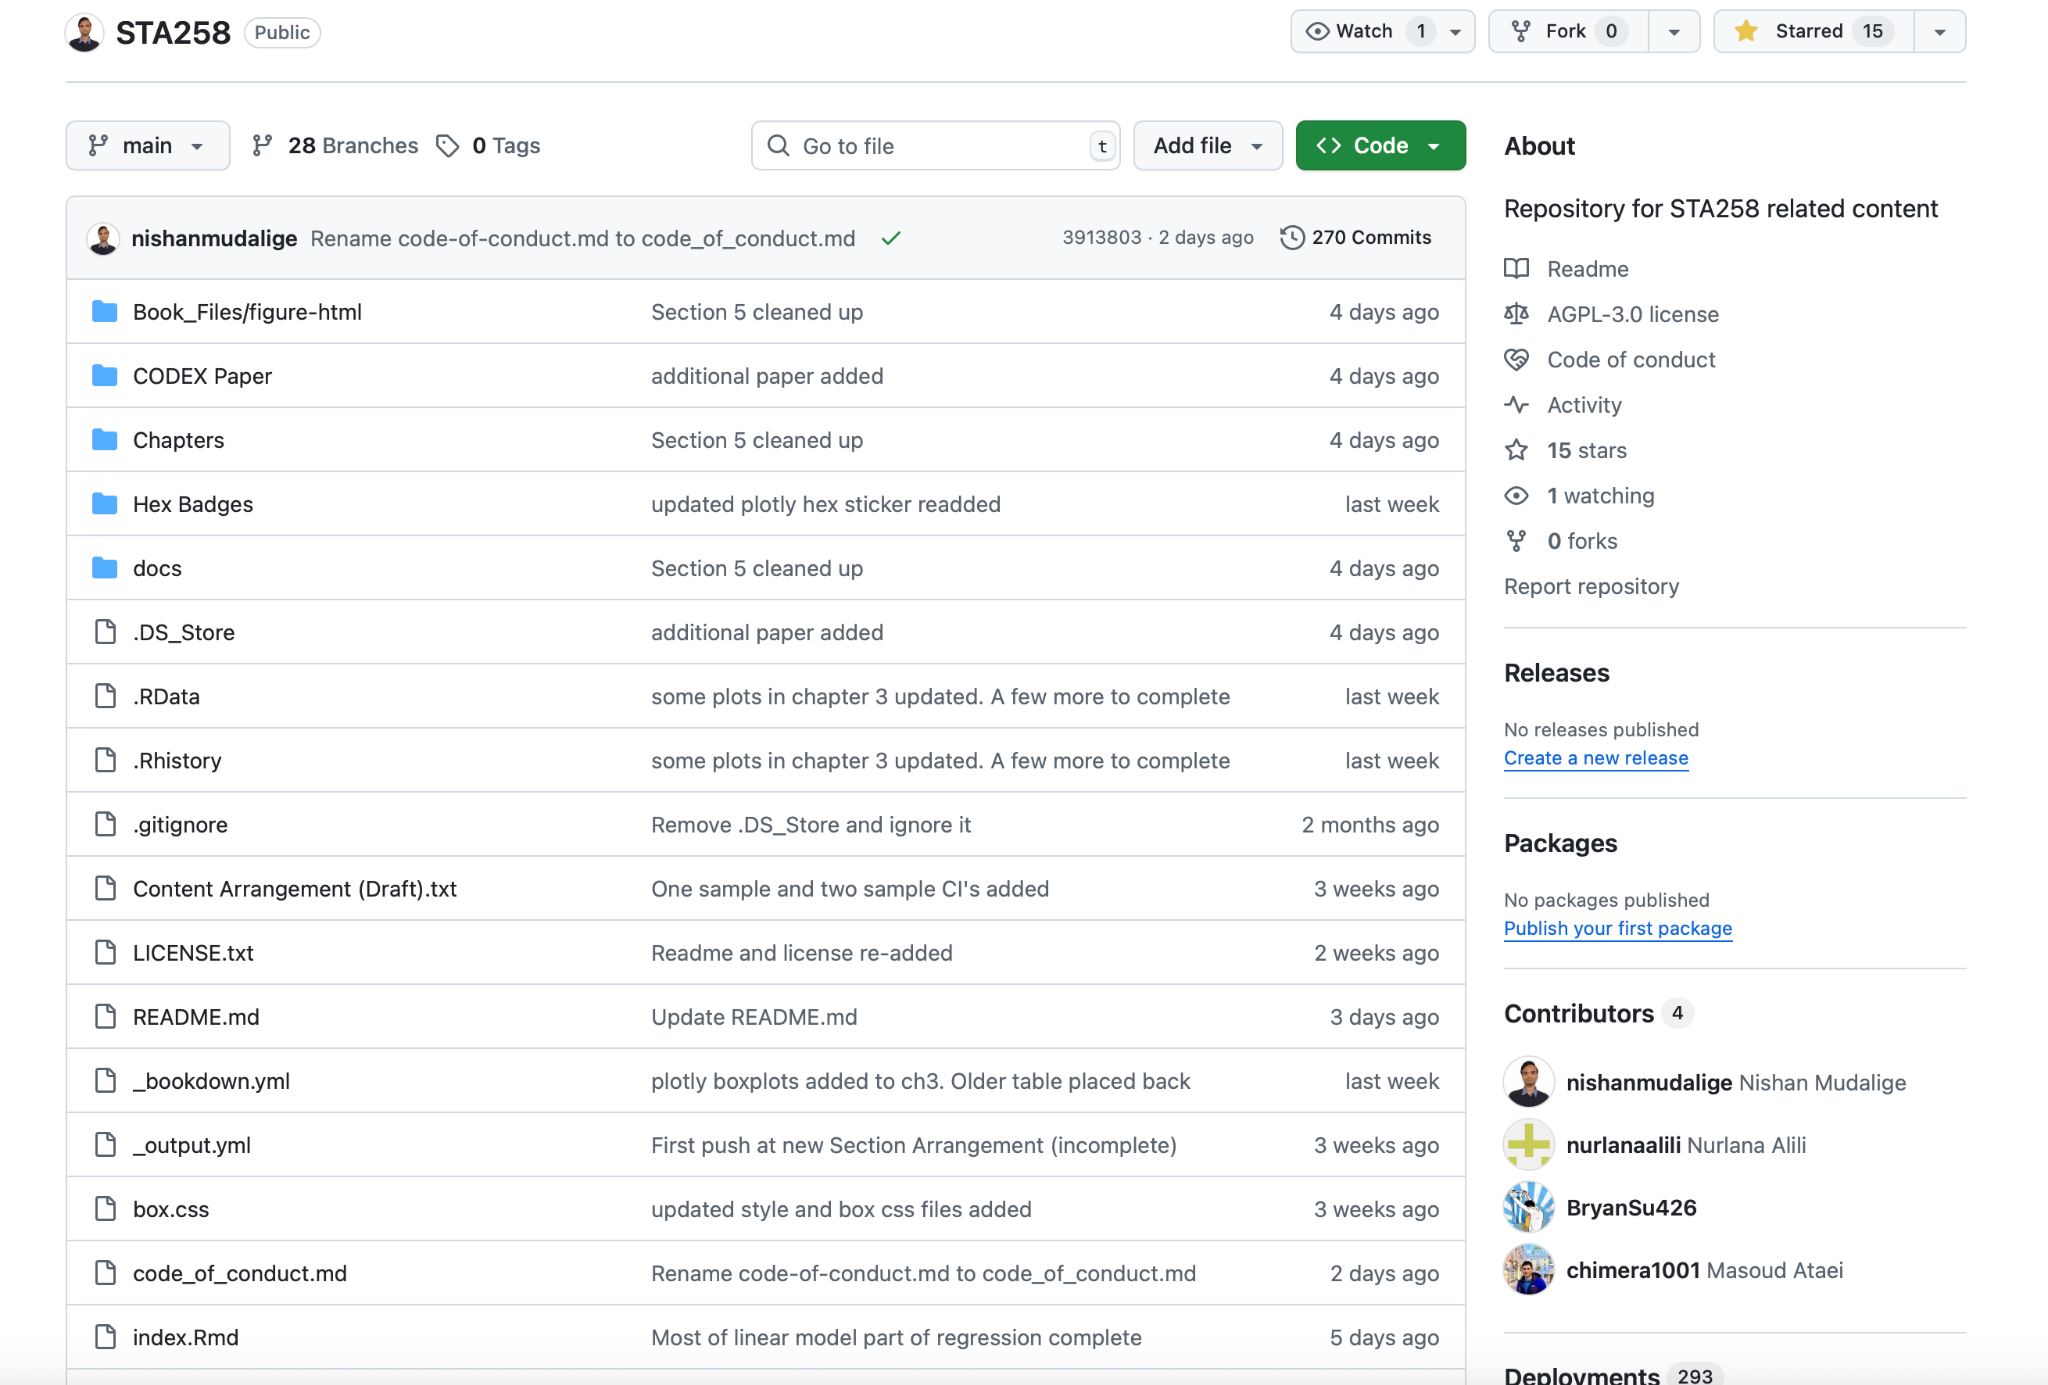
\includegraphics[width=0.7\textwidth]{Images/github-ss.png}
%\end{pepadunfigure}

The development of the e-book required significant planning and coordination to ensure that the final product was cohesive and pedagogically meaningful. The initial draft was largely a collection of lecture notes and presentation slides. 
We used these to build a single unified document which was a one-to-one replication of the notes and slides.
This was our baseline draft for the e-book.
During the development of this baseline, the inclusion of figures and graphics was sparse since we were aware that content would be rearranged.
After reviewing this initial baseline draft, we realized that the large number of chapters resulted in fragmentation of related content, making it difficult for students to learn material.

Through collaboration and discussion, we combined overlapping sections and reordered material into a more logical flow. This process helped reduce redundancy and resulted in a smoother experience for both students and instructors and material being presented in a coherent manner.
We also removed as much content as possible which overlapped with STA260, making these two courses much more distinct.
Once the order and layout were finalized, the content created was rearranged and refined, and static and interactive plots and figures were built around the updated content.

Static and interactive plots and figures are rendered natively within the R Markdown file within code blocks.
An example of a code block used to render a figure using the ggplot2 library is given in Listing \ref{lst:Markdown_ggplot2}.
Interactive plots were created using the Plotly and R Shiny.\\

\begin{lstlisting}[language=R,
                   caption={An example of a code block in Markdown used to render an image with ggplot},
                   label={lst:Markdown_ggplot2},
                   captionpos=b] 
```{r label, fig.cap="Example Code Block", echo=FALSE, fig.align='center', warning=FALSE}
library(ggplot2)

# code for ggplot2 figure goes here
```
\end{lstlisting}

Similar to ggplot2, plotly figures are generated natively within codeblocks.
The Tikz package was initially used with LaTeX to create some graphics used in the both the initial PDF and the Bookdown version of the e-book, since Tikz is a powerful package which can create vector graphics.
However, we discovered that we can create all of the required graphics using ggplot2 and plotly, so we decided to utilize these 2 packages for all figures for a more consistent appearance.
R Shiny apps were developed in R and hosted on \href{https://www.shinyapps.io/}{Shinyapps.io}. 
These apps are natively embedded into the e-book using a code block and some HTML for formatting.
Listing \ref{lst:Markdown_shiny} provides the syntax for embedding R Shiny apps in the e-book.\\

\begin{lstlisting}[language=R,
                   caption={An example of a code block in Markdown used to render an image with ggplot},
                   label={lst:Markdown_shiny},
                   captionpos=b] 
<center>
```{r HistShinyApp, echo=FALSE, out.width='100%', warning=FALSE}
knitr::include_app("URL to App Hosted on shinyapps.io", )
```
</center>
\end{lstlisting}

Finally, we used the rgl library to create a 3D interactive version of the digital hex sticker designed for the project which appears on the cover of the e-book.



\section{CONTENT AND INTERACTIVE DESIGN}

We selected to utilize the default theme of Bookdown since it has a clean layout and appearance.
The default theme also comes with options for light and dark mode and the table of contents appears along the left.
The landing page in light and dark mode are presented in Figure \ref{fig:landing_page}.

\begin{figure}[h!]
    \centering
    \begin{subfigure}[t]{0.5\textwidth}
        \centering
        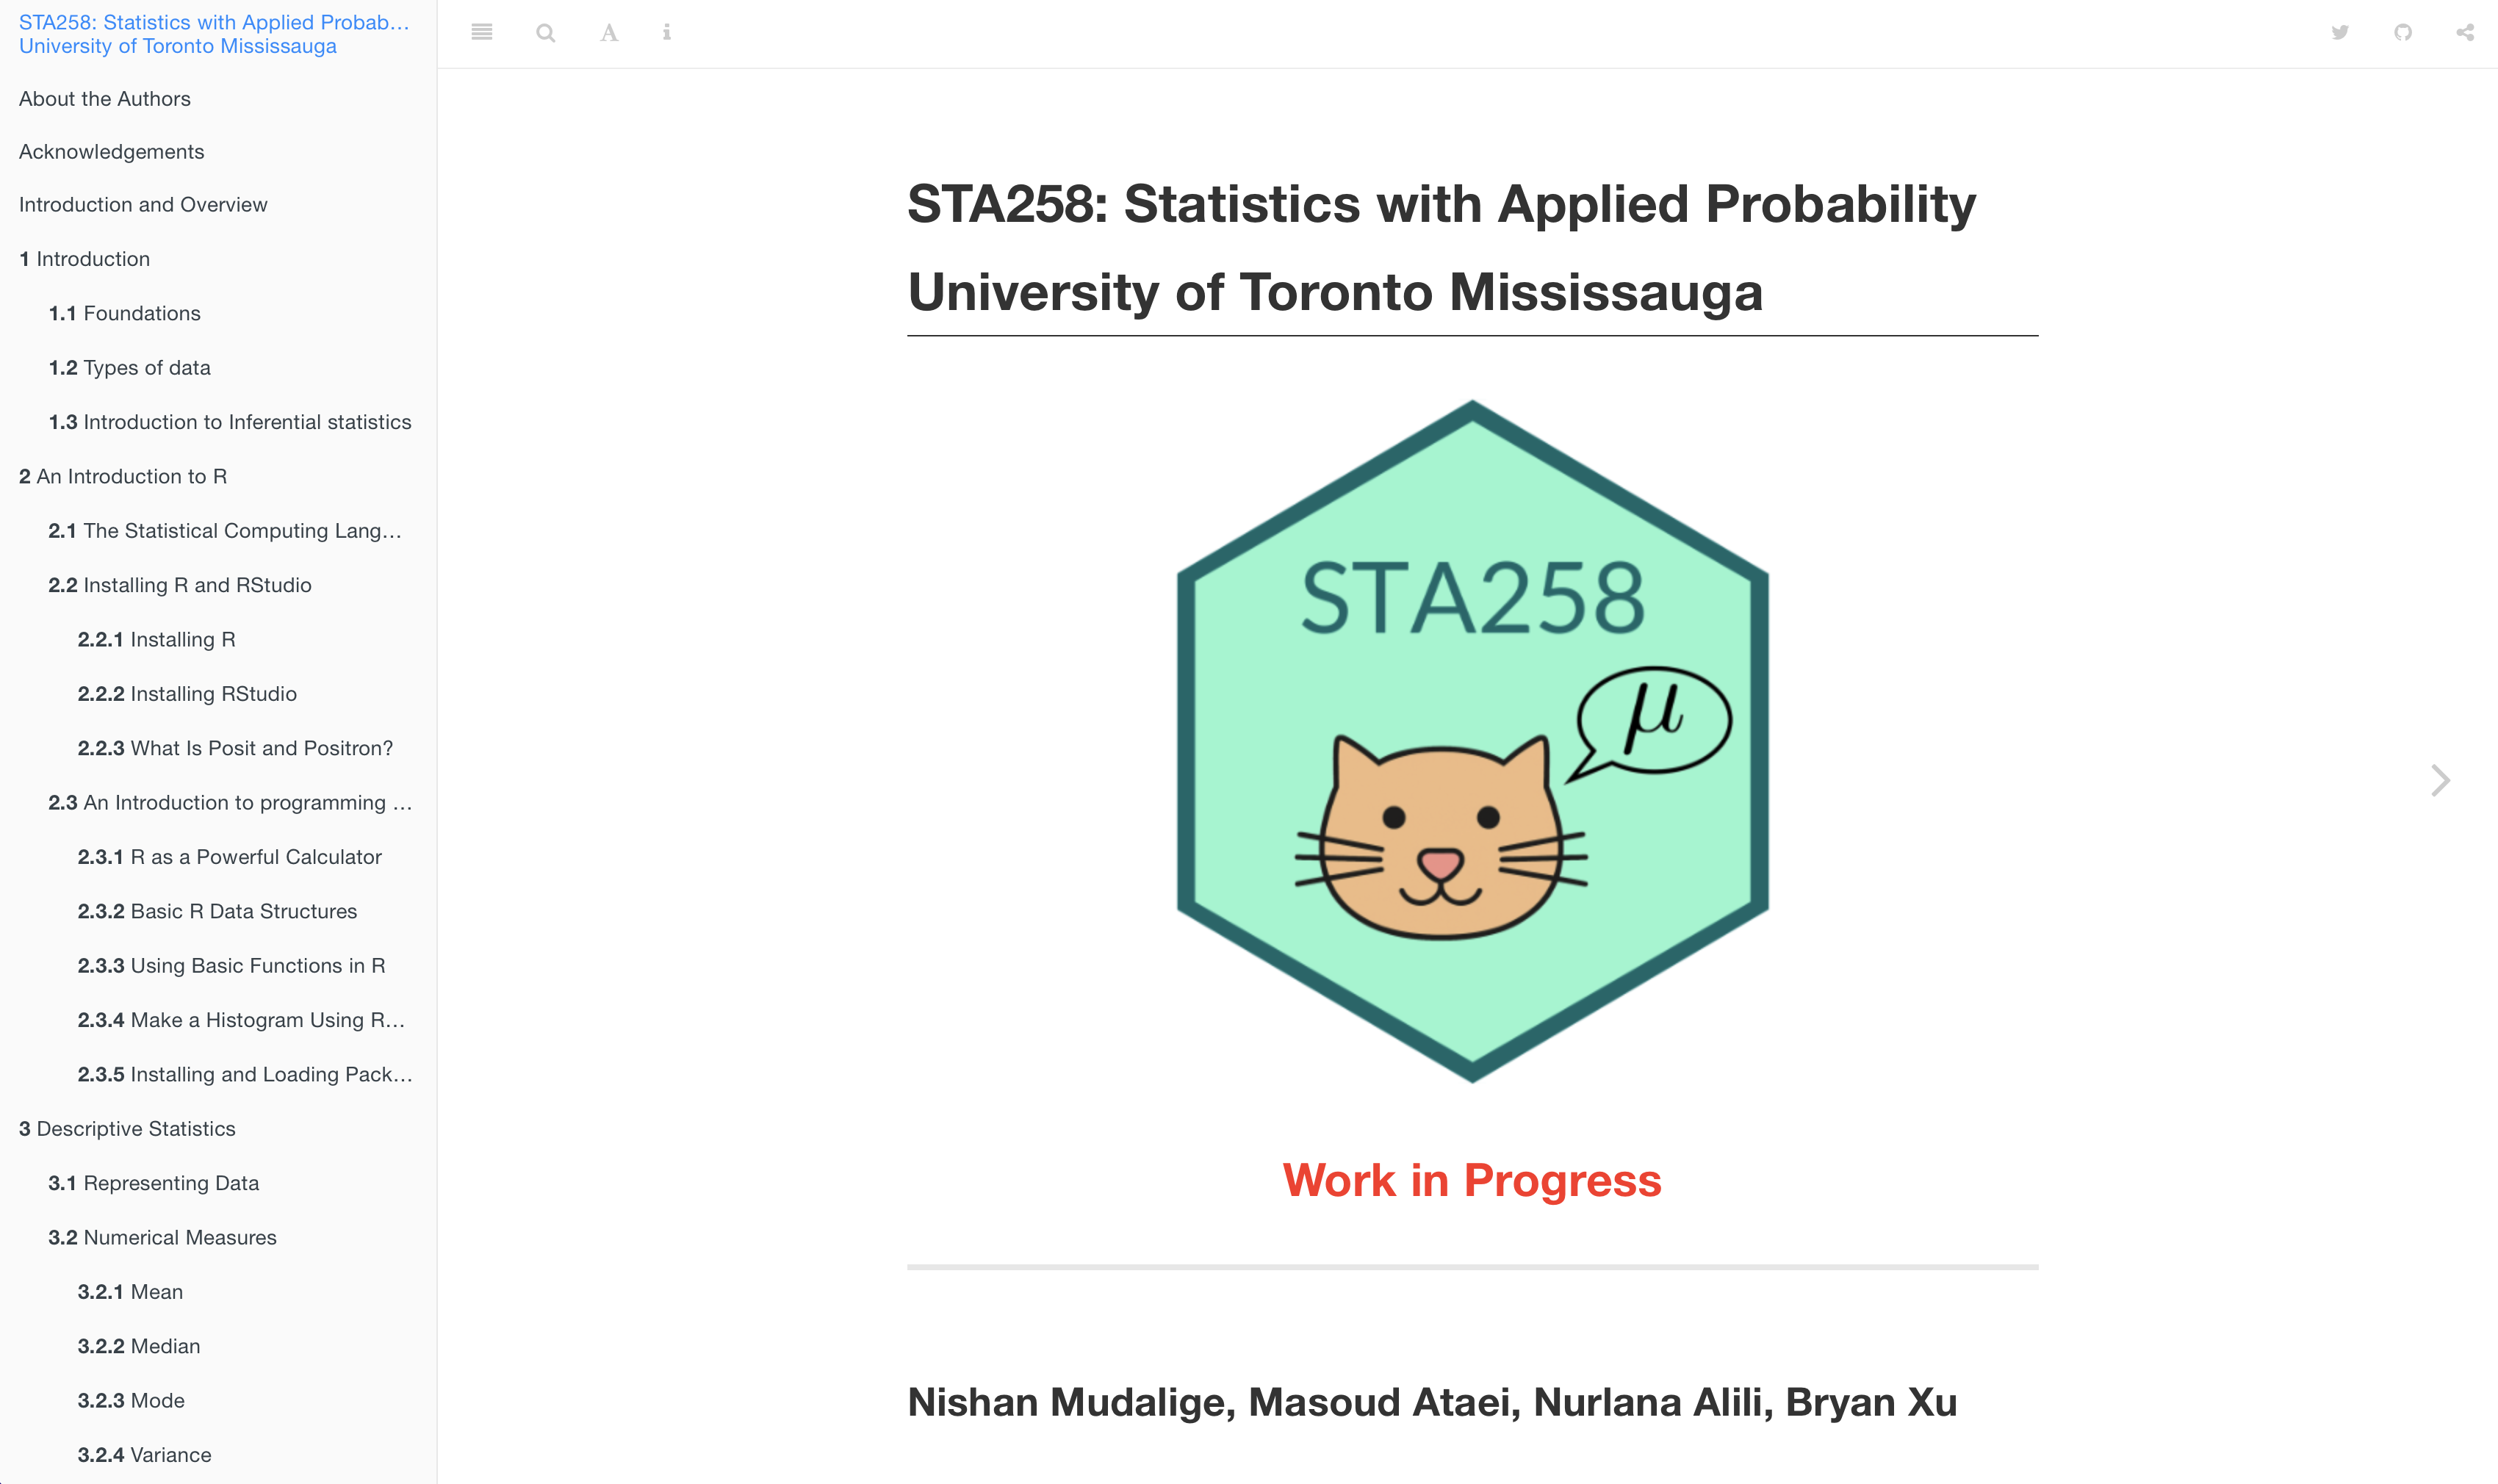
\includegraphics[width=0.975\textwidth]{Images/ebookCover.png}
        \caption{Landing page of the e-book in the default layout.}
    \end{subfigure}%
    \hfill
    \hfill
    \begin{subfigure}[t]{0.5\textwidth}
        \centering
        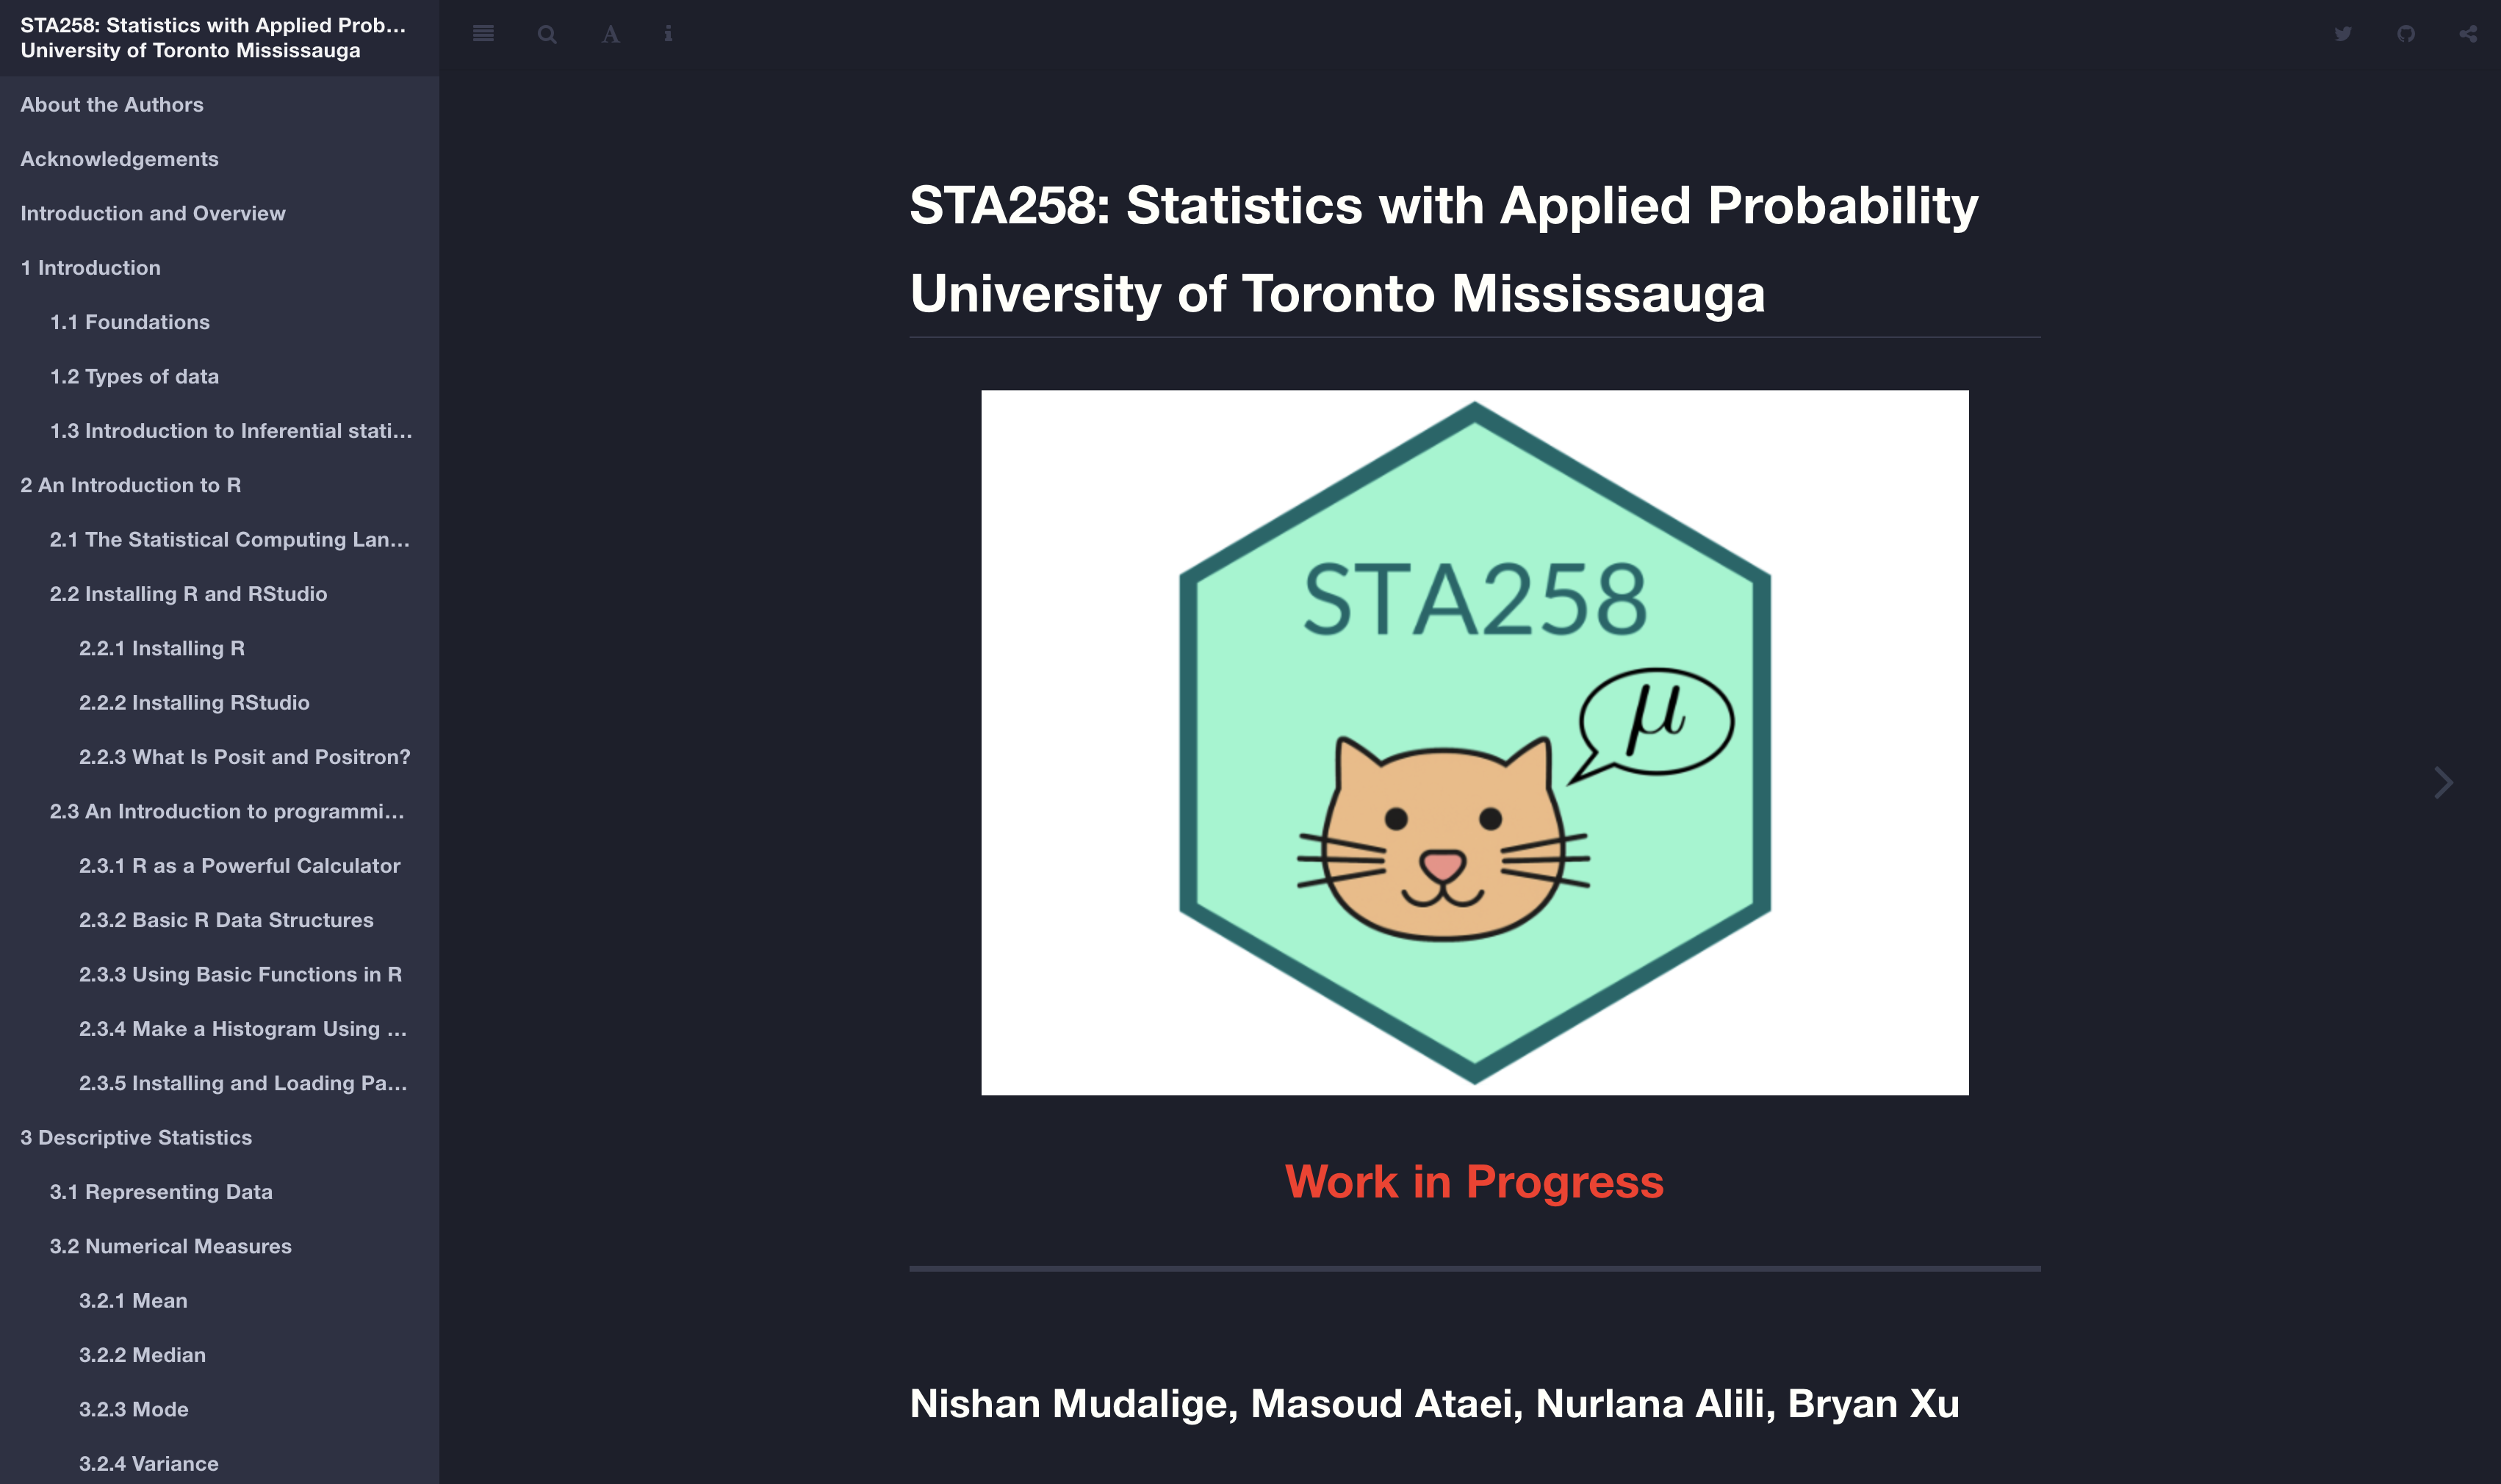
\includegraphics[width=0.975\textwidth]{Images/ebookCover_dark.png}
        \caption{Landing page of the e-book in dark mode.}
    \end{subfigure}
    \caption{Landing page of the e-book in the default and dark theme. Notice the table of contents on the left.}
    \label{fig:landing_page}
\end{figure}

%\begin{pepadunfigure}{GitHub repository structure showing organized files, collaborative development history, and team contributions for the e-book project. GitHub supported version control, content management, and public access through GitHub Pages.}
%    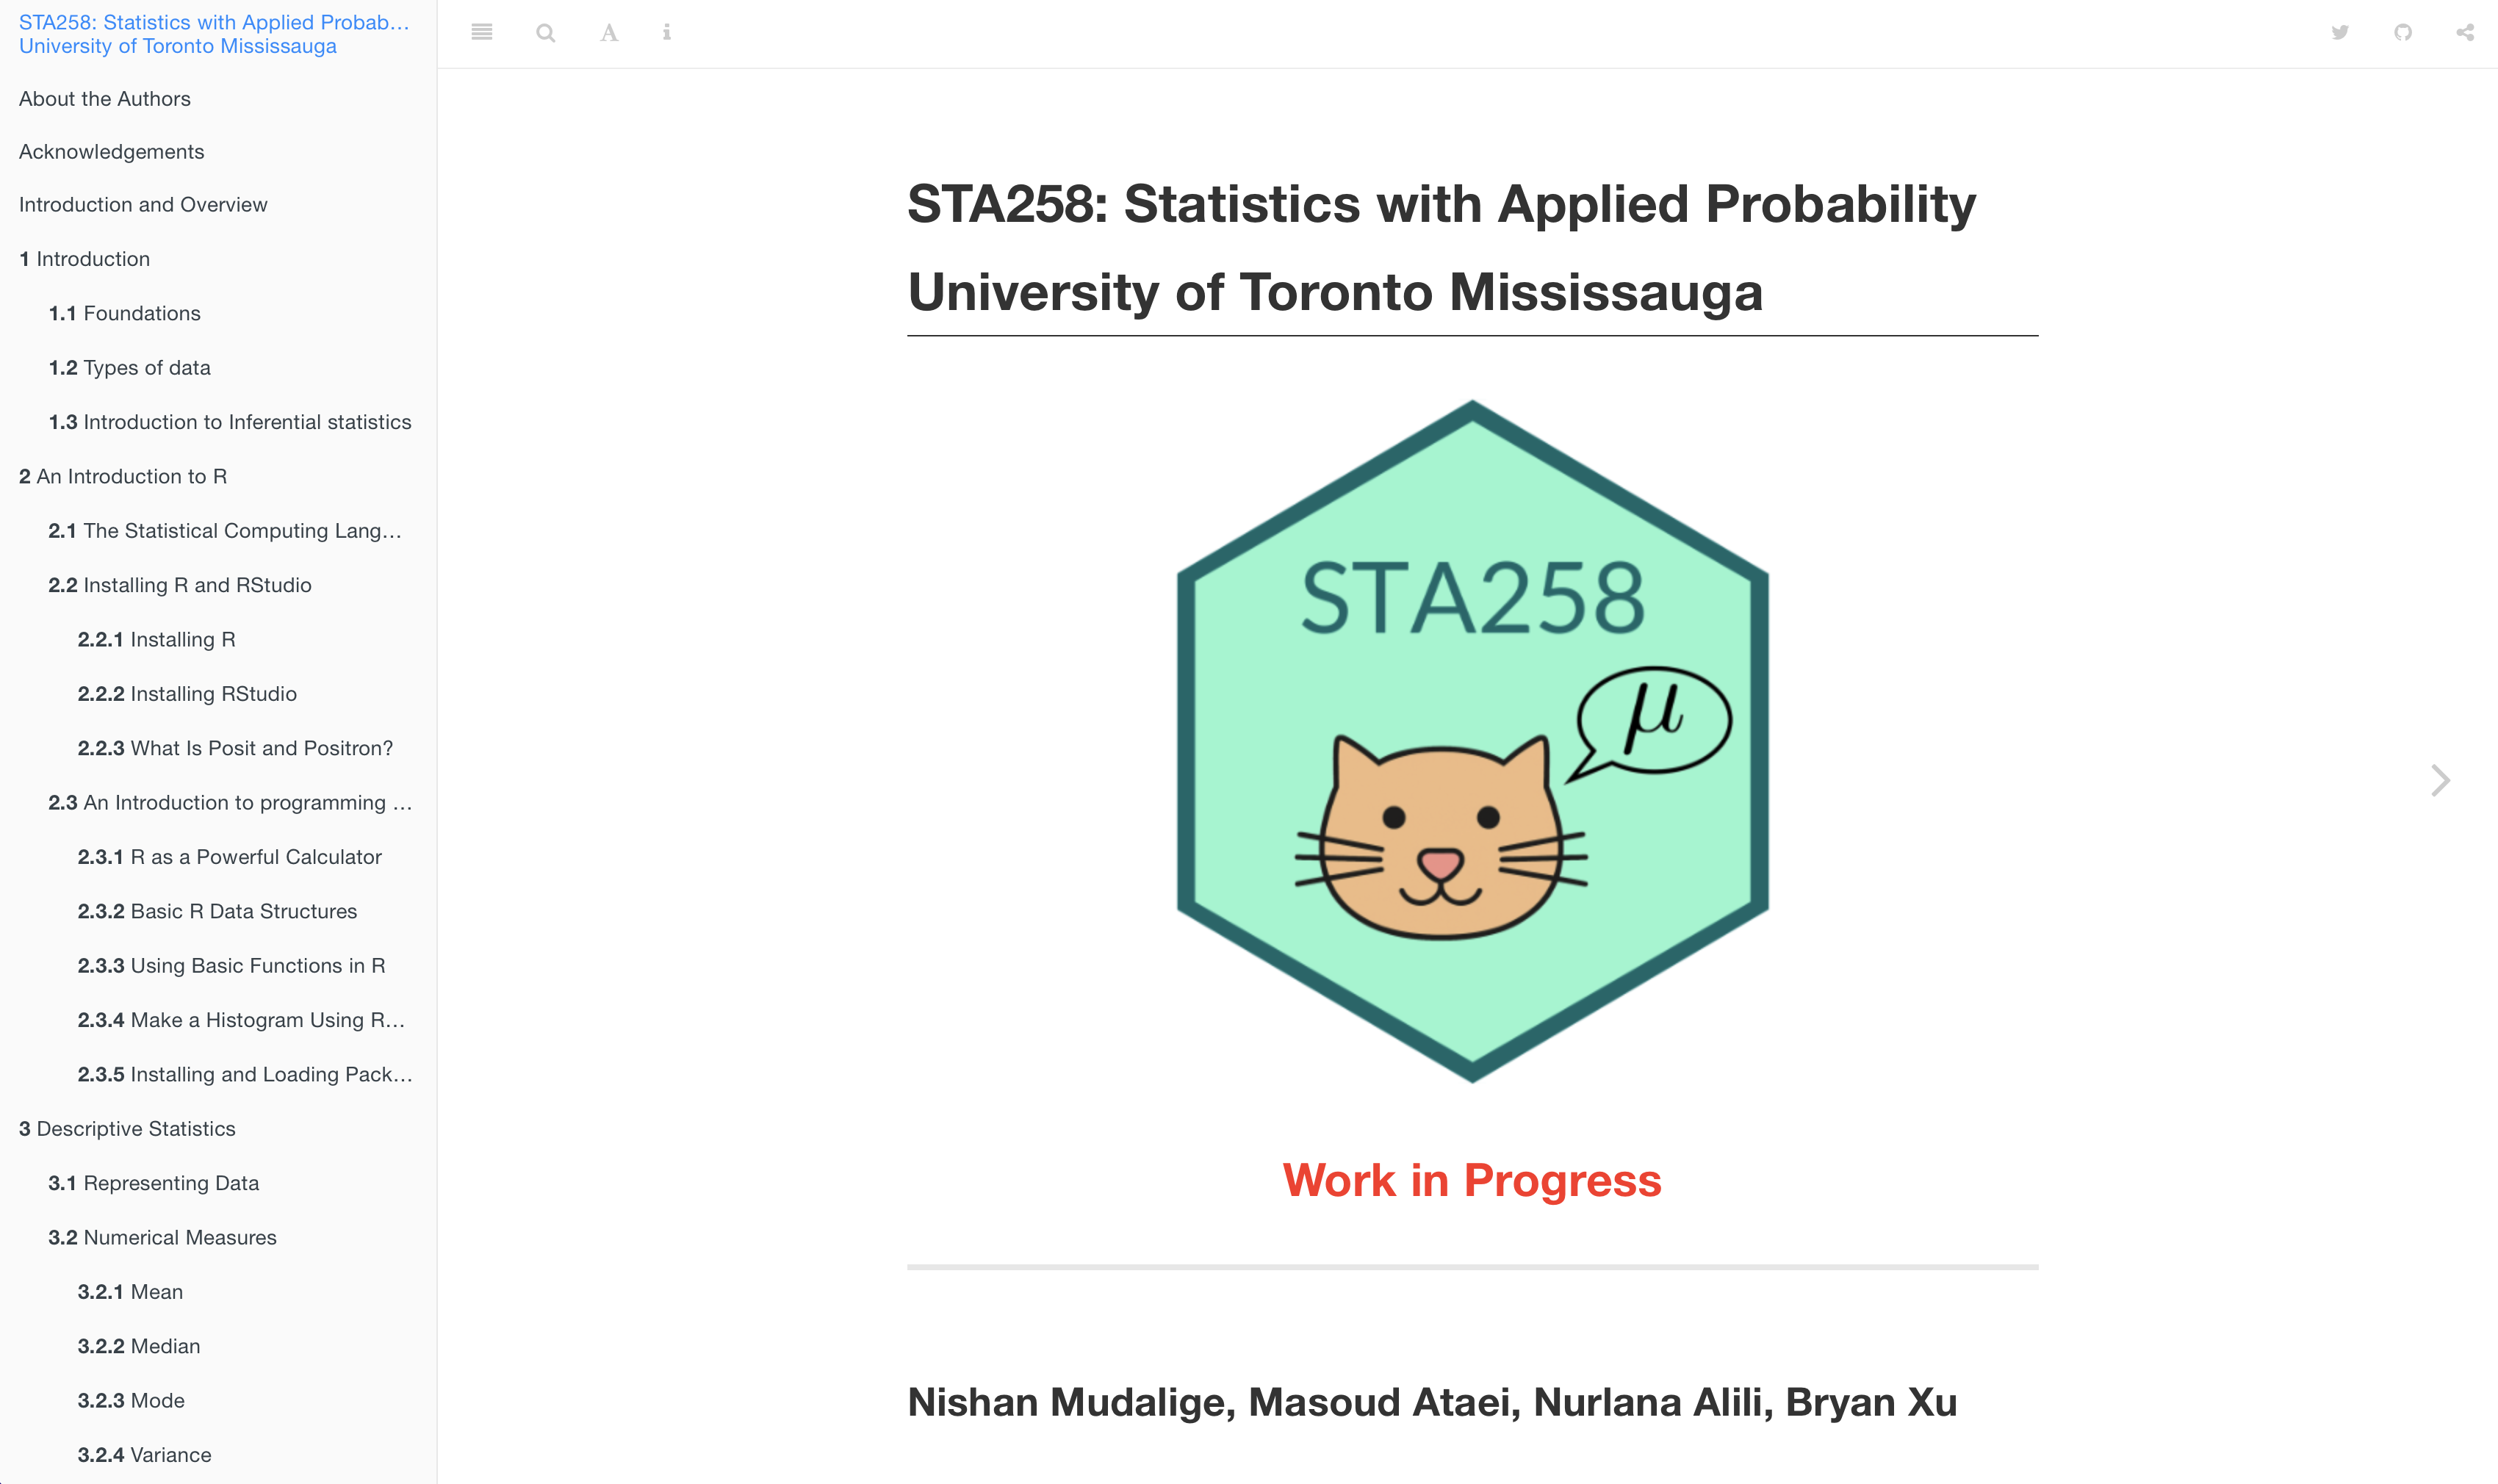
\includegraphics[width=0.7\textwidth]{Images/ebookCover.png}
%\end{pepadunfigure}

The content of the material presented begins with foundational statistical concepts, including key terminology, data types, and the basic ideas behind inferential statistics. Recognizing the importance of technical skills, we included an early chapter on R programming and its practical uses. This section explains how to install R, use essential functions, and work with basic data structures and visualizations. Together, these elements provide a strong technical foundation. From there, the book progresses through core statistical methods, covering confidence intervals, hypothesis testing, and statistical power, before moving into topics such as analysis of variance, linear regression, and categorical data analysis. The structure was designed to support progressive skill-building for students while offering instructors a clear and teachable sequence of topics.

One of the most challenging aspects of the project was presenting statistical ideas visually in a way that was both accurate and engaging. At first, we used TikZ in LaTeX to create static diagrams, which worked well for simple illustrations. However, more complex concepts, such as how changes in correlation affect the shape of data, were difficult to represent using only static figures. While we could explain the theory behind these concepts, the lack of interactivity limited students’ ability to explore them meaningfully.

After encountering this limitation, we revisited our approach to visualization. We shifted to using R Markdown and Shiny to build interactive web applications. These tools allowed students to manipulate variables and observe how distributions changed in real time. Although they took time to build and required trial and error, they significantly improved the exploratory aspect of the learning experience.

To illustrate these interactive elements in practice, we developed a short lesson on histogram interpretation, skewness, and dynamic bin width adjustment. This section begins by comparing left-skewed, right-skewed, and symmetric distributions using interactive histograms, helping students build intuition about shape and spread. The lesson concludes with an app that allows students to adjust bin widths and explore how histogram appearance changes with sampling resolution (Figures 2–5).

\begin{figure}[H]
  \centering
  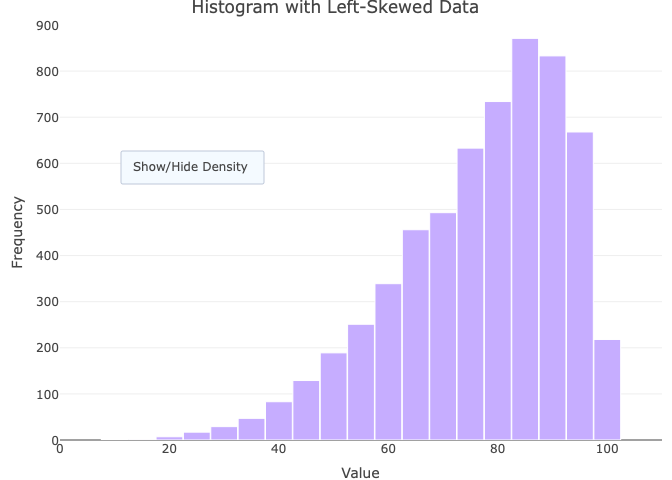
\includegraphics[width=0.75\textwidth]{Images/left.png}
  \caption{An interactive histogram displaying a left-skewed distribution. Students can toggle the kernel density overlay and observe how left-skewness shifts the bulk of the distribution toward higher values, providing a visual interpretation of negative skew.}
\end{figure}

\begin{figure}[H]
  \centering
  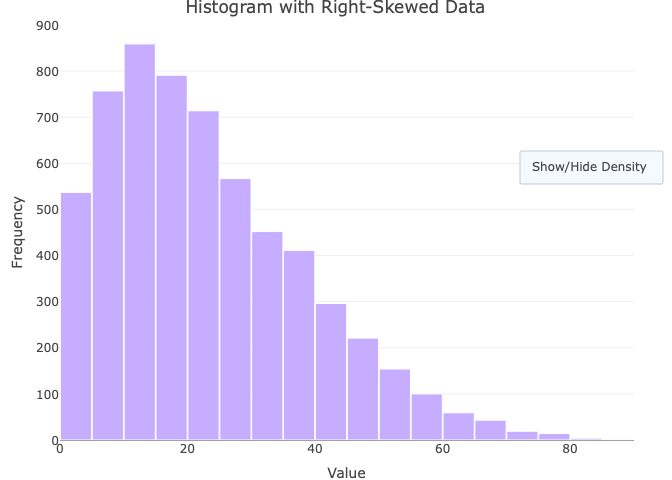
\includegraphics[width=0.75\textwidth]{Images/right.png}
  \caption{A histogram showing a right-skewed distribution. This figure enables students to identify how the majority of values cluster on the left side, with a long tail extending rightward, reinforcing the concept of positive skew.}
\end{figure}

\begin{figure}[H]
  \centering
  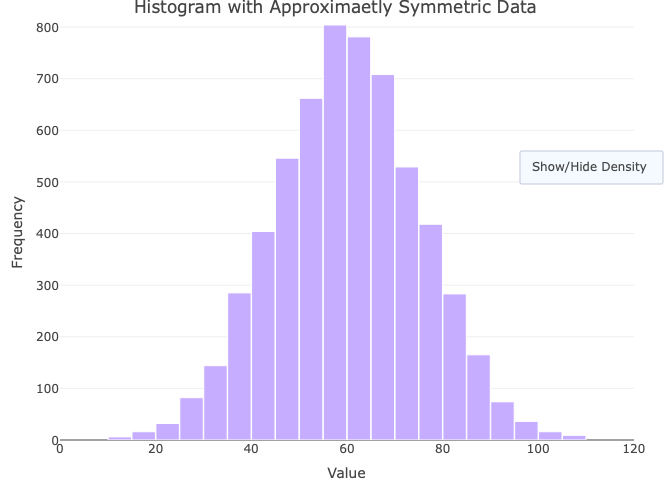
\includegraphics[width=0.75\textwidth]{Images/symm.png}
  \caption{A symmetric histogram used to contrast with skewed examples. It illustrates an approximately normal distribution with balanced tails, aiding in comparisons of central tendency and dispersion.}
\end{figure}

\begin{figure}[H]
  \centering
  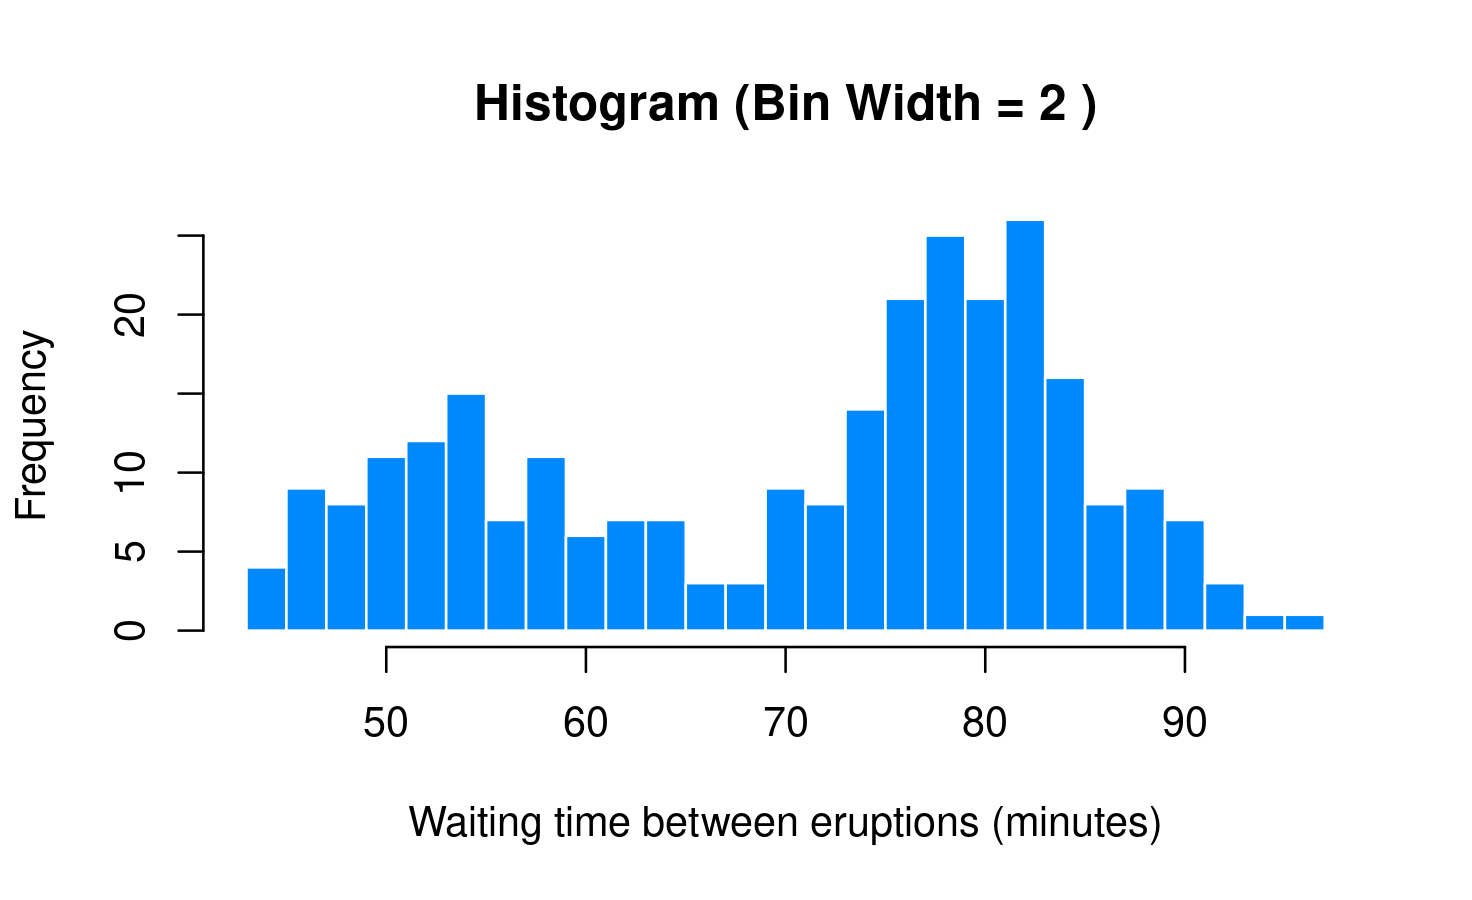
\includegraphics[width=0.75\textwidth]{Images/bin.png}
  \caption{Interactive application that allows students to adjust the bin width for a histogram built on real-world data (geyser eruption waiting times). The tool demonstrates how histogram appearance is sensitive to graphical parameters, enhancing students’ understanding of distribution shape and granularity.}
\end{figure}


One of the most rewarding parts of the project was designing the figures. Many were created using ggplot2 and are now central features of the e-book. They are visually clear, carefully styled, and interactive where appropriate. These visualizations reflect intentional design choices and help communicate complex ideas in a way that is both intuitive and accessible. Although this process was time-consuming, it was also one of the most enjoyable and educational parts of the project.

\begin{figure}[H]
  \centering
  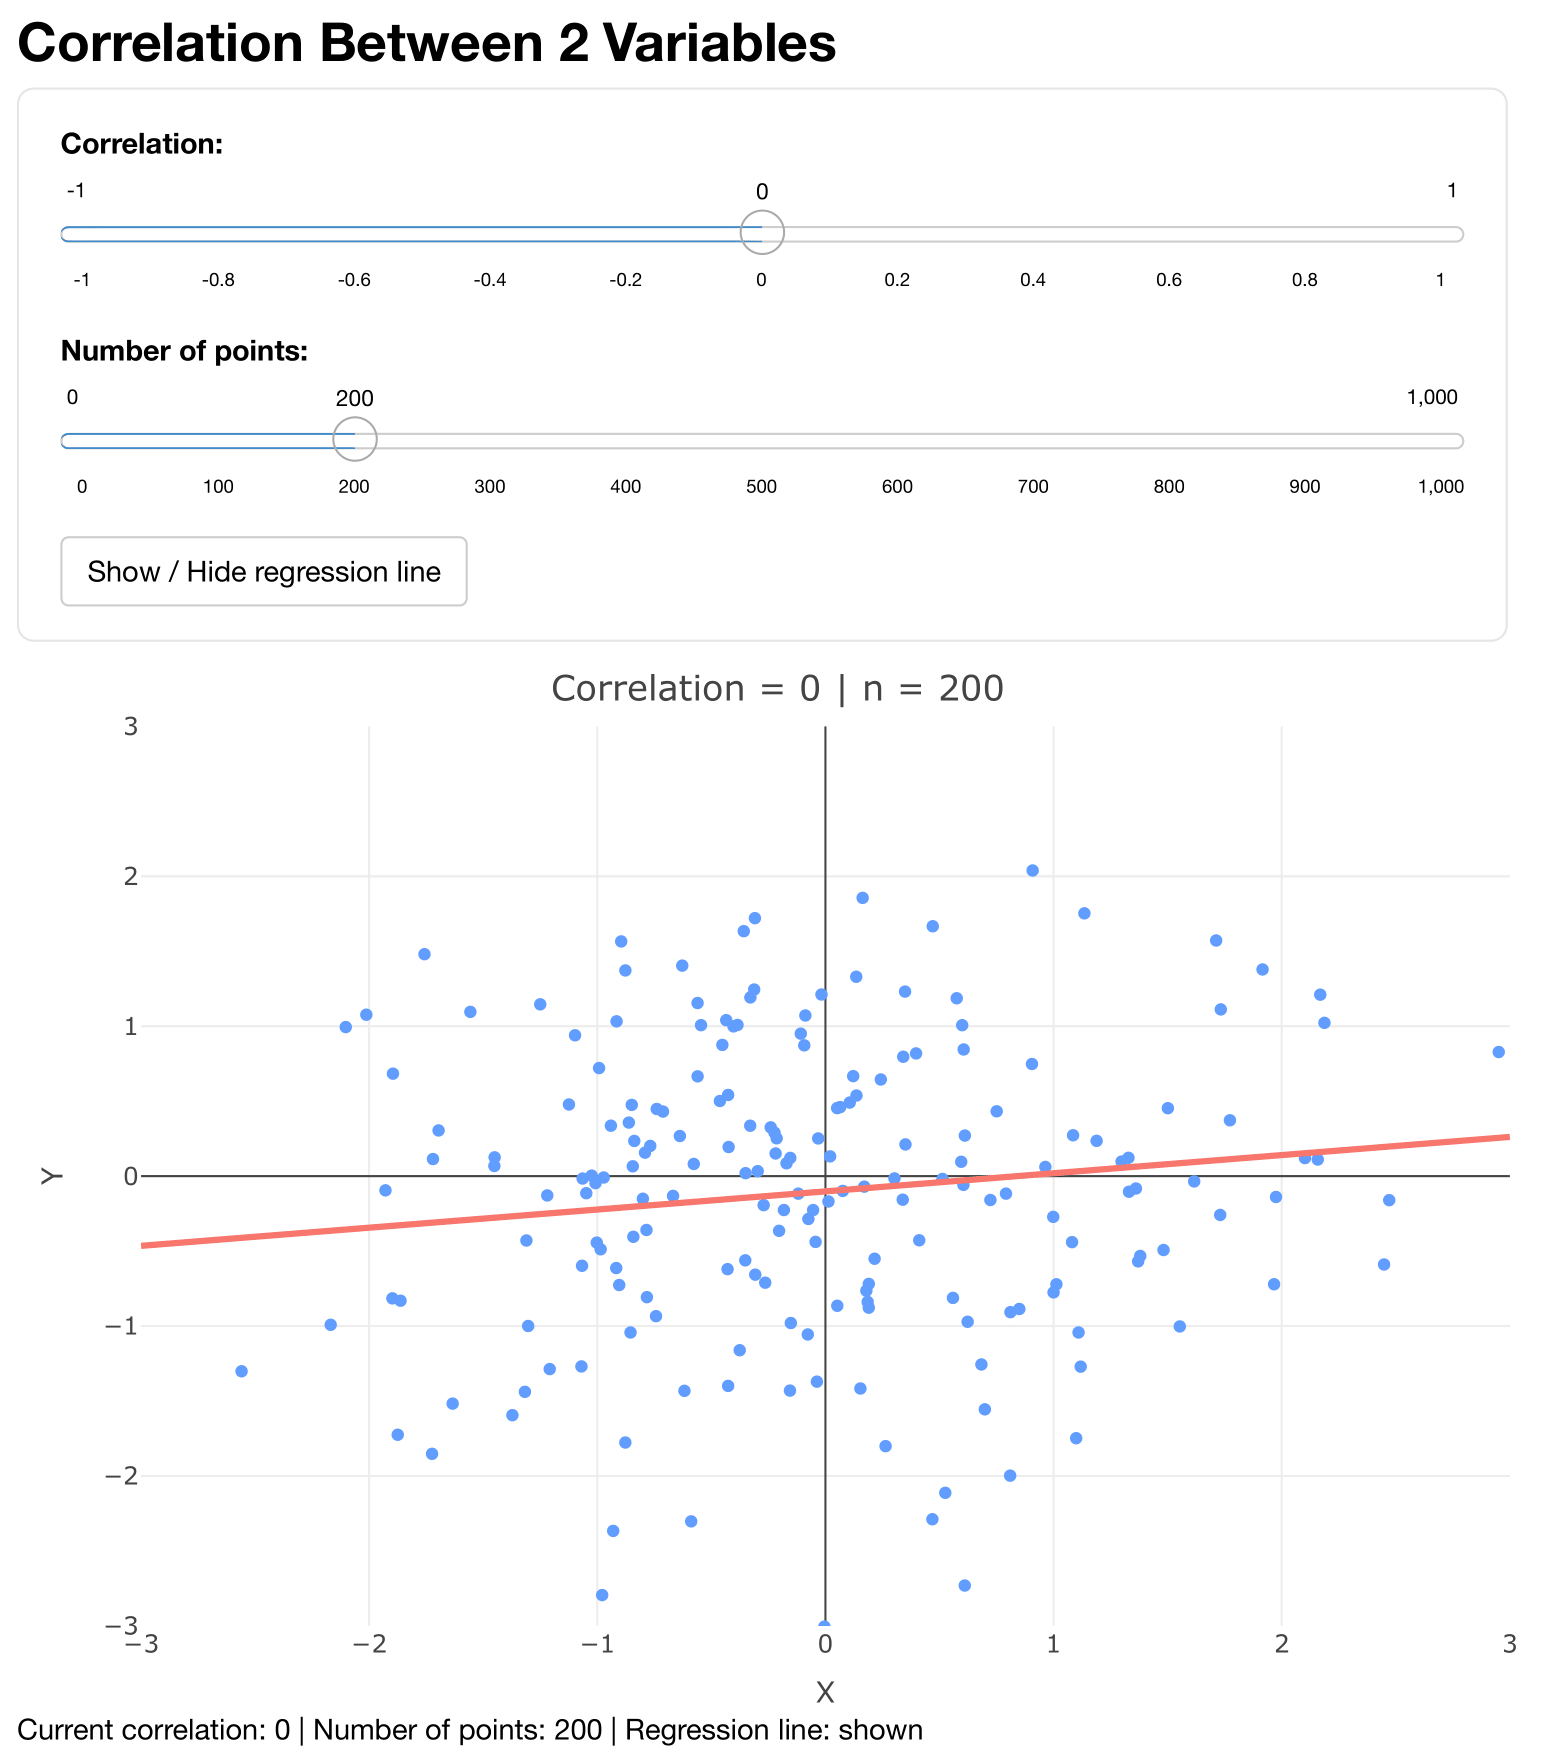
\includegraphics[width=0.7\textwidth]{Images/ch9-image.png}
  \caption{Interactive Shiny app exploring the relationship between two variables at varying correlation levels. Users can dynamically adjust the correlation coefficient and sample size, and optionally display the regression line. This tool helps students visualize how correlation strength influences the spread and direction of data points, reinforcing conceptual understanding through real-time feedback.}
\end{figure}


\section{CONCLUSION}

Beyond its technical and instructional outcomes, this project demonstrates the pedagogical potential of student-led authorship and design. By actively participating in the creation of educational content, students shift from consumers to contributors of knowledge, engaging more deeply with the subject matter.

The process required not only statistical expertise and programming fluency, but also adaptability, design thinking, and critical reflection—skills applicable in both academic and professional contexts. Through collaborative authorship, the final product embodies negotiated decisions, iterative problem-solving, and responsiveness to peer and faculty feedback.

More broadly, the project presents a replicable model of participatory curriculum development that integrates open-source tools, student initiative, and faculty mentorship to generate accessible, engaging, and adaptive learning resources.

\section{FUTURE WORK}

While the current version of the e-book successfully integrates core statistical ideas with interactive elements, there are several directions for future development. One important area is expanding the content to include more advanced topics, such as generalized linear models, non-parametric tests, or multivariate analysis. Including these topics would make the resource more useful for students in upper-year or specialized courses.

Improving accessibility and the overall user experience is another key goal. Possible next steps include optimizing the interface for mobile devices, adding text-to-speech functionality, and offering multilingual options. These features would help the e-book reach a wider range of learners from diverse backgrounds.

From a technical perspective, future versions could explore more extensive use of Shiny dashboards, where students would be able to interact with full datasets and generate real-time statistical outputs within the textbook. Additional features, such as embedded quizzes, automatic feedback on code, and user-submitted notes, could further enhance student engagement and retention of concepts.

In the long term, we hope to maintain and grow the project through continued collaboration between students and faculty. Building a clear versioning system, contributor documentation, and a guide for future authors would help ensure that the e-book remains a living resource that evolves with each new cohort.


\begin{acknowledgments}
We would like to sincerely thank Professor Nishan Mudalige, who served as the principal supervisor for this project from the very beginning. His guidance, encouragement, and consistent support played a central role in shaping both the direction and success of the e-book.

We are also grateful to Professor Masoud Ataei, whose input during the later stages of development helped refine both the technical and pedagogical aspects of the project. His feedback was thoughtful and valuable throughout.

We thank our fellow collaborators for their contributions and support, as well as the Department of Mathematical and Computational Sciences at the University of Toronto Mississauga for fostering an environment where student–faculty collaboration is encouraged and actively supported and facilitated.

Finally, we acknowledge the open-source community. The tools, documentation, and shared knowledge developed and maintained by contributors around the world made the technical side of this project achievable and rewarding.
\end{acknowledgments}

%────────────────────────────────────────────────
%— Updated bibliography command
\printbibliography[title={REFERENCES},heading=bibintoc]

\end{document}
